\section{Maximum likelihood estimation}
\label{sec:ch6:mle}

When you learned about random networks which can be described using single network models, one of the key things we covered were the *parameters* that define the underlying random networks. If you see a network in practice and want to learn about it, you have to make sets of assumptions. One of these assumptions you made in the preceding chapter, namely, is that the network is a sample of a random network, which obeys particular rules as to how it behaves. However, you have a slight problem, because learning about an underlying random network *requires* us to have some understanding of the parameters that define it. What are you to do?


\subsection{Erd\"os-R\'enyi (ER)}

Recall that the Erd\"os-R\'enyi (ER) random network has a single parameter: the probability of each edge existing, which we termed $p$. Due to the simplicity of an ER random network, we can resort to a technique called Maximum Likelihood Estimation (MLE), through which you can obtain a reasonable guess at $p$, which for various reasons, is desirable. You can look at the appendix {numref}`app:ch13:mle` for justification for the utility of this estimator, and check out \cite{Casella2001Jun} for more details on maximum likelihood estimation.

We'll develop some intuition for this procedure by going back to our coin flip example. You have a coin, for which you don't know the probability it lands on heads is. However, you are told you can flip that coin, and after $100$ flips, you have to guess what the probability of heads is for the coin. For instance, if you flip the coin $100$ times, and it lands on heads $45$ times, what would you guess that the probability the coin lands on heads would be?

If you thought to yourself that you would guess $\frac{45}{100}$, which is just the ratio of the number of heads that you saw to the total number of coin flips, you would have a pretty good estimate. This is called the maximum likelihood estimate of the probability for a binary (heads or tails, $1$ or $0$) random variable. For the ER random network, this works exactly the same way. You find that the best estimate of the probability of an edge existing in an ER random network is just the ratio of the total number of edges in the network, $m = \sum_{j > i}a_{ij}$, divided by the total number of edges possible in the network, which is $\binom n 2$.

Our result is:
\begin{align*}
    \hat p &= \frac{m}{\binom n 2}.
\end{align*}

All the ``hat'' symbol ($\hat \cdot $) means is that $\hat p$ it is an \textit{estimator}: it is a function of the observed data that we use to describe the \textit{estimand}, which is the parameter of the model that we want to learn about. In this case, since we are considering an $ER_n(p)$ model, the only parameter that we want to learn about is $p$.

To bring this back to our coin flip example, this is like you are saying that there is a single coin. You flip the coin once for every possible edge between those pairs of communities, $\binom n 2$. When that coin lands on heads, that particular edge is determined to exist, and when it lands on tails, that edge does not exist. Our best guess, then, is just to count the number of heads you obtained, $m$, and divide by the number of coin flips you made, $\binom n 2$. 

Let's work on an example. You will use a sample of a random network which is ER, with $50$ nodes and an edge probability of $0.3$, similar to what we did in Section \ref{sec:ch5:er}. We begin by simulating and visualizing the appropriate network: 


\begin{lstlisting}[style=python]
from graspologic.simulations import er_np

p = 0.3
A = er_np(n=50, p=p)
\end{lstlisting}

Next, we'll fit the appropriate model from \texttt{graspologic}, and compare the true probability $p=0.3$ to the estimated probability $\hat p$:
\begin{lstlisting}[style=python]
import numpy as np
from graspologic.models import EREstimator

model = EREstimator(directed=False, loops=False)
model.fit(A)
# obtain the estimate from the fit model
phat = model.p_
\end{lstlisting}

We can see how good the estimator performs by comparing it to the (true) population parameter, $p$:

\begin{lstlisting}[style=python]
print("Difference between phat and p: {:.3f}".format(phat - p))
\end{lstlisting}

Not bad! The estimate of the probability should end up pretty close to the true value. 

\subsection{Stochastic Block Model}

The Stochastic Block Model also has a single parameter: the block matrix, $B$, whose entries $b_{kk'}$ denote the probabilities of edges existing or not existing between pairs of communities in the Stochastic Block Model. When you apply the method of MLE to the SBM, what you find is that, where $m_{kk'}$ is the total number of edges between nodes in communities $k$ and $k'$, and $n_{kk'}$ is the number of edges possible between nodes in communities $k$ and $k'$:

\begin{align*}
    \hat b_{kk'} = \frac{m_{kk'}}{n_{kk'}}.
\end{align*}

Intuitively, the estimate of the block probability $b_{kk'}$ is the ratio of how many edges you see between communities $k$ and $k'$ $m_{kk'}$ and how many edges were possible $n_{kk'}$.

To bring this back to our coin flip example, this is like you are saying that there is one coin called coin $(k, k')$ for each pair of communities in our network. You flip each coin once for every possible edge between those pairs of communities, $n_{kk'}$. When that coin lands on heads, that particular edge is determined to exist, and when it lands on tails, that edge does not exist. Our best guess, then, is just to count the number of heads you obtained, $m_{kk'}$, and divide by the number of coin flips you made, $n_{kk'}$. 

Remember that in the example we worked through in {numref}`ch5:sbm`, you had $100$ students, each of whom were in one of two schools (school $1$ and school $2$). If the students were both in school $1$, the probability that they were friends was $0.6$, and if the students were both in school $2$, the probability that they were friends was $0.4$. If the students attended different schools, the probability that they were friends was $0.2$. This gave us a block matrix of:
\begin{align*}
    B &= \begin{bmatrix}
        .6 & .2 \\
        .2 & .4
    \end{bmatrix}
\end{align*}

Which corresponds to a probability matrix $P$ where each entry is:
\begin{align*}
    p_{ij} &= \begin{cases}
    0.8 & i, j \leq 20 \text{ or }i, j \geq 20 \\
    0.2 & \text{otherwise}
    \end{cases}
\end{align*}

We begin by simulating an appropriate SBM:

\begin{lstlisting}[style=python]
from graspologic.simulations import sbm

n = [50, 50]
B = np.array([[0.6, 0.1], 
              [0.1, 0.4]])

A = sbm(n=n, p=B)
z = [0 for i in range(0,n[0])] + [1 for i in range(0, n[1])]
\end{lstlisting}

A network sample is shown in Figure \ref{fig:ch5:sbm}.

Next, let's fit an appropriate SBM, and investigate the estimate of $B$:

\begin{lstlisting}[style=python]
from graspologic.models import SBMEstimator
from graphbook_code import heatmap

model = SBMEstimator(directed=False, loops=False)
model.fit(A, y=z)
Bhat = model.block_p_

# plot the block matrix vs estimate
heatmap(B, title=" $B$ true block matrix")
heatmap(Bhat, title="$\hat B$ estimate of block matrix")
heatmap(np.abs(Bhat - B), title="$|\hat B - B|$")
\end{lstlisting}

We investigate the difference between $B$ and $\hat B$ in Figure \ref{fig:ch6:sbm_est}.

\begin{figure}
    \centering
    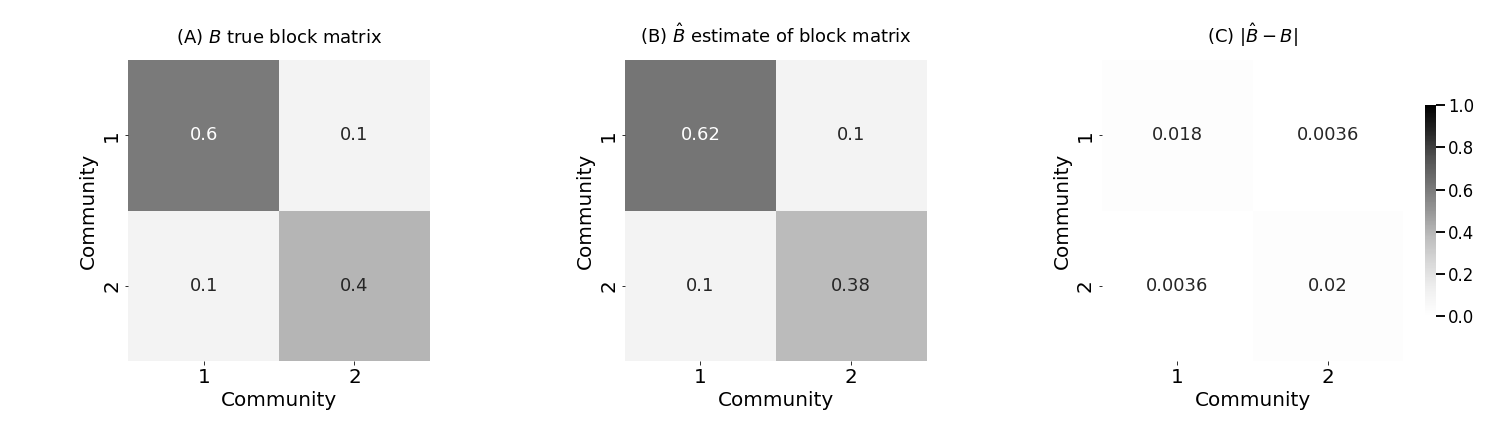
\includegraphics[width=\linewidth]{representations/ch6/Images/sbm_est.png}
    \caption[Estimating block matrix of SBM]{\textbf{(A)} the true block matrix underlying a random network. \textbf{(B)} the estimated block matrix from the network sample. \textbf{(C)} the difference between the estimated and true block matrices.}
    \label{fig:ch6:sbm_est}
\end{figure}

So, from what we have learned here, when we have extremely simple networks in which we think that it's reasonable to conceptualize the edges in the network as largely untsructured (the $ER_n(p)$ random network case) or that the structure in the network can be completely described by a community assignment that we know ahead of time (the $SBM_n(\vec z, B)$ case, in which we only need to learn about $B$), we can obtain fairly good estimates of the underlying probability parameters of the models.

\newpage